\documentclass[twocolumn,nofootinbib,showkeys,twoside,floatfix,unsortedaddress,flushbottom,10pt,aps,pra]{report}
\input  4mbapreamble
\usepackage{tikz}
\usepackage{latexsym}% 
\usepackage{graphics,graphicx}
\usepackage{amssymb}% 
\usepackage{amsmath}
\usepackage{amsfonts} % mathbb
\usepackage{natbib}% 
\usepackage{fancyhdr,lastpage}
\usepackage{titlesec}
%\usepackage[margin=0.7in,headheight=60pt]{geometry}
\usepackage[width = 18cm, height = 22cm,headheight=60pt, columnsep = 1cm]{geometry}

\usepackage{lipsum}% http://ctan.org/pkg/lipsum
\usepackage{float}
\usepackage{listings}
\usepackage{subfigure}
\usetikzlibrary{shapes.geometric, arrows}
\tikzset{
  int/.style={circle, draw=black, fill=blue!20, minimum size=3em},
  init/.style={pin distance=1.2cm,pin edge={loop,thin,black}}
}
\tikzstyle{arrow} = [thick,black,->,>=stealth]
\tikzstyle{pinstyleto} = [pin edge={<-,thick,black}]
\tikzstyle{pinstyleout} = [pin edge={->,thick,black}]


\newcommand\numberthis{\addtocounter{equation}{1}\tag{\theequation}}
%\newcommand{\R}{{\cal R}}
%\newcommand{\Rlogo}{\protect
\includegraphics[height=2ex,keepaspectratio]{images/Rlogo.pdf}\xspace}

\AtBeginDocument{%
\renewcommand{\thesection}{\arabic{section}}%
\renewcommand{\contentsname}{\sc{Contents}}
\renewcommand{\bibname}{\sc{Bibilography}}
}
\author{\sc{Model Students:}\\
 \small \emph{Melody Fong} \\
 \small \emph{Nicole Dumont} \\
 \small  \emph{Carolina Weishaar}}
 \title{ \small \emph{Mathematics 4MB3/6MB3: Mathematical Biology }\\
  \Huge \sc{Spatial Epidemics Dynamics:\\ Synchronization}}
  \date{\today}
  

%\renewcommand{\abstractname}{\Huge \sc{Executive Summary}}

  \titleformat{\section}
  {\centering \normalfont \scshape}{\thesection}{1em}{}
  
  \titleformat{\subsection}
  {\centering \normalfont \itshape}{\thesubsection}{1em}{}



\lhead{\sc{Synchronization}}
\rhead{\emph{Model Students}} 
\renewcommand\headrulewidth{0pt}% Removes funny header line
\begin{document}



\pagestyle{fancy}

\maketitle
\tableofcontents

\onecolumn
\section*{\Huge Executive Summary}
\addcontentsline{toc}{section}{\protect\numberline{}Executive Summary}%
\lipsum[34]

\twocolumn

\section{Abstract} Text goes here.
\section{Literature Review }
In recent years there has been an increased awareness of the threat posed by various high profile diseases, such as SARS, Ebola and Influenza \cite{Liu2009}. Long-term incidence records of such diseases exhibit recurrent epidemics illustrated by homogeneous and heterogeneous cycles. In the presence of control health care measures, such as vaccination, the peaks of these cycles do dampen out yet persist \cite{Lloyd1996}. Due to the complex set of social and biological structures involved in this interaction, mathematical models provide an excellent framework in which the eradication of long-term recurrence can be studied \cite{Sattenspiel2009}. \par

To accomplish this goal, many mathematical models have been derived on the basis of the migration of an individual through the various stages of an epidemic, however these models have failed to illustrate the recurrent nature of these diseases \cite{Lloyd2004}. One observable biological factor neglected by many of these models is the notion of spatial dynamics. Classically it has been assumed that susceptible and infectious individuals are distributed uniformly within a population. However, incidence records clearly show that this long-term recurrent behaviour is sustained through through the spatial dynamics that facilitate the spread of disease between sub populations experiencing an outbreak and disease free sub populations. As a result, to model recurrent oscillations it is essential that the disease dynamics of a  population is represented by the set of interactions between local homogeneous populations \cite{Earn2000}.\par

In order to account for spatial heterogeneity, this study considers a meta-population model, where a population is divided into several discrete sub classes, called patches, each exhibiting a well dispersed population. The population representing a patch is modelled by the susceptible, infectious and removed (SIR) model where each individual belongs to either the susceptible, infectious, or removed class. The state of the system changes according to the rates that allow an individual to migrate between classes. In addition to this, this study makes use of sinusoidal seasonal forcing on the transmission rate, in order to accurately depict the observed variation in the number of individuals that enter the infectious class on an annual basis based on various social parameters. The SIR model exhibits two equilibrium points whose stability is determined by the basic reproduction number $\R_0$. If  $\R_0 > 1$, the system approaches an endemic equilibrium via damped oscillations \cite{Lloyd1996}. Otherwise, the system approaches a disease free equilibrium. The aim of this study is to analyze the dynamics of this model overtime, in order to determine which parameter values lead the synchronization of all patches, thereby generating a disease free state exhibited by the entire population. \par

\section{Methods}
\subsection{The Metapatch SIR Model} 
The spatial SIR model consists of $n$ identical patches (which represent cities or some other spatial grouping of people) with identical population sizes. The population is constant in each patch and there is no migration between patches. Intra-patch dynamics are given by the standard SIR model with vital dynamics and sinusoidal seasonal forcing. Connectivity between patches is represented by disease transmission. Infected individuals can infect people from other patches. This models individuals visiting other patches, creating additional sources of infection in the visited patch. 
A visualization of the dynamics in a single patch $i$ is shown by
\begin{center}
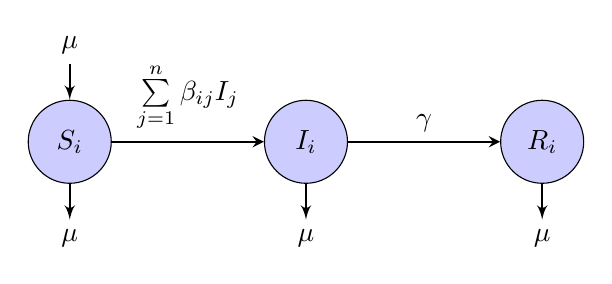
\begin{tikzpicture}[node distance=3cm,auto,>=latex',every node/.append style={align=center}]
    \node [int, pin={[pinstyleto]above:$\mu$}, pin={[pinstyleout]below:$\mu$}] (a)              {$S_i$};
    \node [int, pin={[pinstyleout]below:$\mu$}] (b) [right of=a] {$I_i$};
    \node [int, pin={[pinstyleout]below:$\mu$}] (c) [right of=b] {$R_i$};
    
    \draw [arrow] (a) -- node[anchor=south] {$ \sum\limits_{j=1}^{n}\beta_{ij} I_j $} (b);
    \draw [arrow] (b) -- node[anchor=south] {$\gamma$} (c);
\end{tikzpicture}
\end{center}

The equations describing the dynamics in a single patch are
\begin{align*}
  \frac{dS_i}{dt} &= \mu - S_i\sum\limits_{j=1}^{n}\beta_{ij}(t) I_j -\mu S_i \\ 
  \frac{dI_i}{dt} &= S_i\sum\limits_{j=1}^{n}\beta_{ij}(t) I_j -\gamma I_i - \mu I_i  \numberthis \label{model} \\
  \frac{dR_i}{dt} &= \gamma I_i -\mu R_i      
\end{align*}
where $S$ is the proportion of the population that is susceptible to infection, $I$ is the proportion of the population that is infectious, and $R$ is the proportion of the population that has recovered from the disease (and  have lifelong immunity) or who have died as a result of the disease. $\mu$ is the birth/death rate, $\gamma$ is the recovery rate, and $\beta_{ij}(t)$ are the elements of the $n\times n$ matrix $\beta(t)$:
\begin{equation}
  \beta(t) = \left < \beta \right > (1+\alpha \cos(2\pi t))M
\end{equation}
$\left < \beta \right > (1+\alpha \cos(2\pi t))$ is the standard sinusoidal forced transmission rate. $M$ is a matrix describing the connectivity between patches. Its $(i,j)$ element is the fraction of time infected individuals from patch $i$ spend visiting $j$. The off-diagonal elements are generally less than the diagonal elements since it is usually assumed individuals spend most of their time in their own patch. $M$ is assumed here to be symmetric - i.e. patch $i$ has as much contact with patch $j$ as $j$ does with $i$. The column sums of $M$ (and thus the rows sums too) are all equal to one - i.e. $M$ is doubley stochastic. This means that all of an individual's time is accounted for.
Two different types of $M$ matrices are used in this paper. The first is equal coupling where all patches are equally connected, i.e. all off-diagonal elements of $M$ are equal. The fraction of time individuals spend outside their own patch is given by the parameter $m$.
\[
M =
\begin{bmatrix}
  1-m & \frac{m}{n-1} & \frac{m}{n-1} & \frac{m}{n-1} \\
  \frac{m}{n-1} & 1-m & \frac{m}{n-1} & \frac{m}{n-1}  \\
  \frac{m}{n-1} & \frac{m}{n-1} & 1-m &  \\
  \frac{m}{n-1} &  &  & \ddots 
\end{bmatrix}
\]
The second motif is nearest neighbor coupling. In this case it is assumed that the patches reside on a ring and people can only visit their two nearest neighbors.
\[
M =
\begin{bmatrix}
  1-m & \frac{m}{2} & 0 & 0 & \dots & \frac{m}{2} \\
  \frac{m}{2} & 1-m & \frac{m}{2} & 0 & & \vdots \\
  0 & \frac{m}{2} & 1-m &  \\
  0 & 0 & & \ddots \\
  \vdots & & & & \ddots & \frac{m}{2} \\
  \frac{m}{2} &  & & \dots & \frac{m}{2} & 1-m \ 
\end{bmatrix}
\]

\subsection{Stochastic Simulations} 

\section{Results}
\subsection{Periods of Single Patch Model }
A bifurcation diagram was created using \verb|XPPAUT|.
This produces a bifurcation diagram which shows the periodic recurrence patterns for the simulated deterministic model of the epidemic pattern. As shown in Figure \ref{fig:bifurcation}, there is a single period 1 orbit for $\{5<\R_0\}\cap\{\R_0>27\}$ as well as a single period 2 orbit for $15<\R_0<25$ and mixed dynamics elsewhere.
\begin{figure}[H]
    \caption{A bifurcation diagram for the single patch sinusoidal forced SIR model.}
    \label{fig:bifurcation}
    \centering
    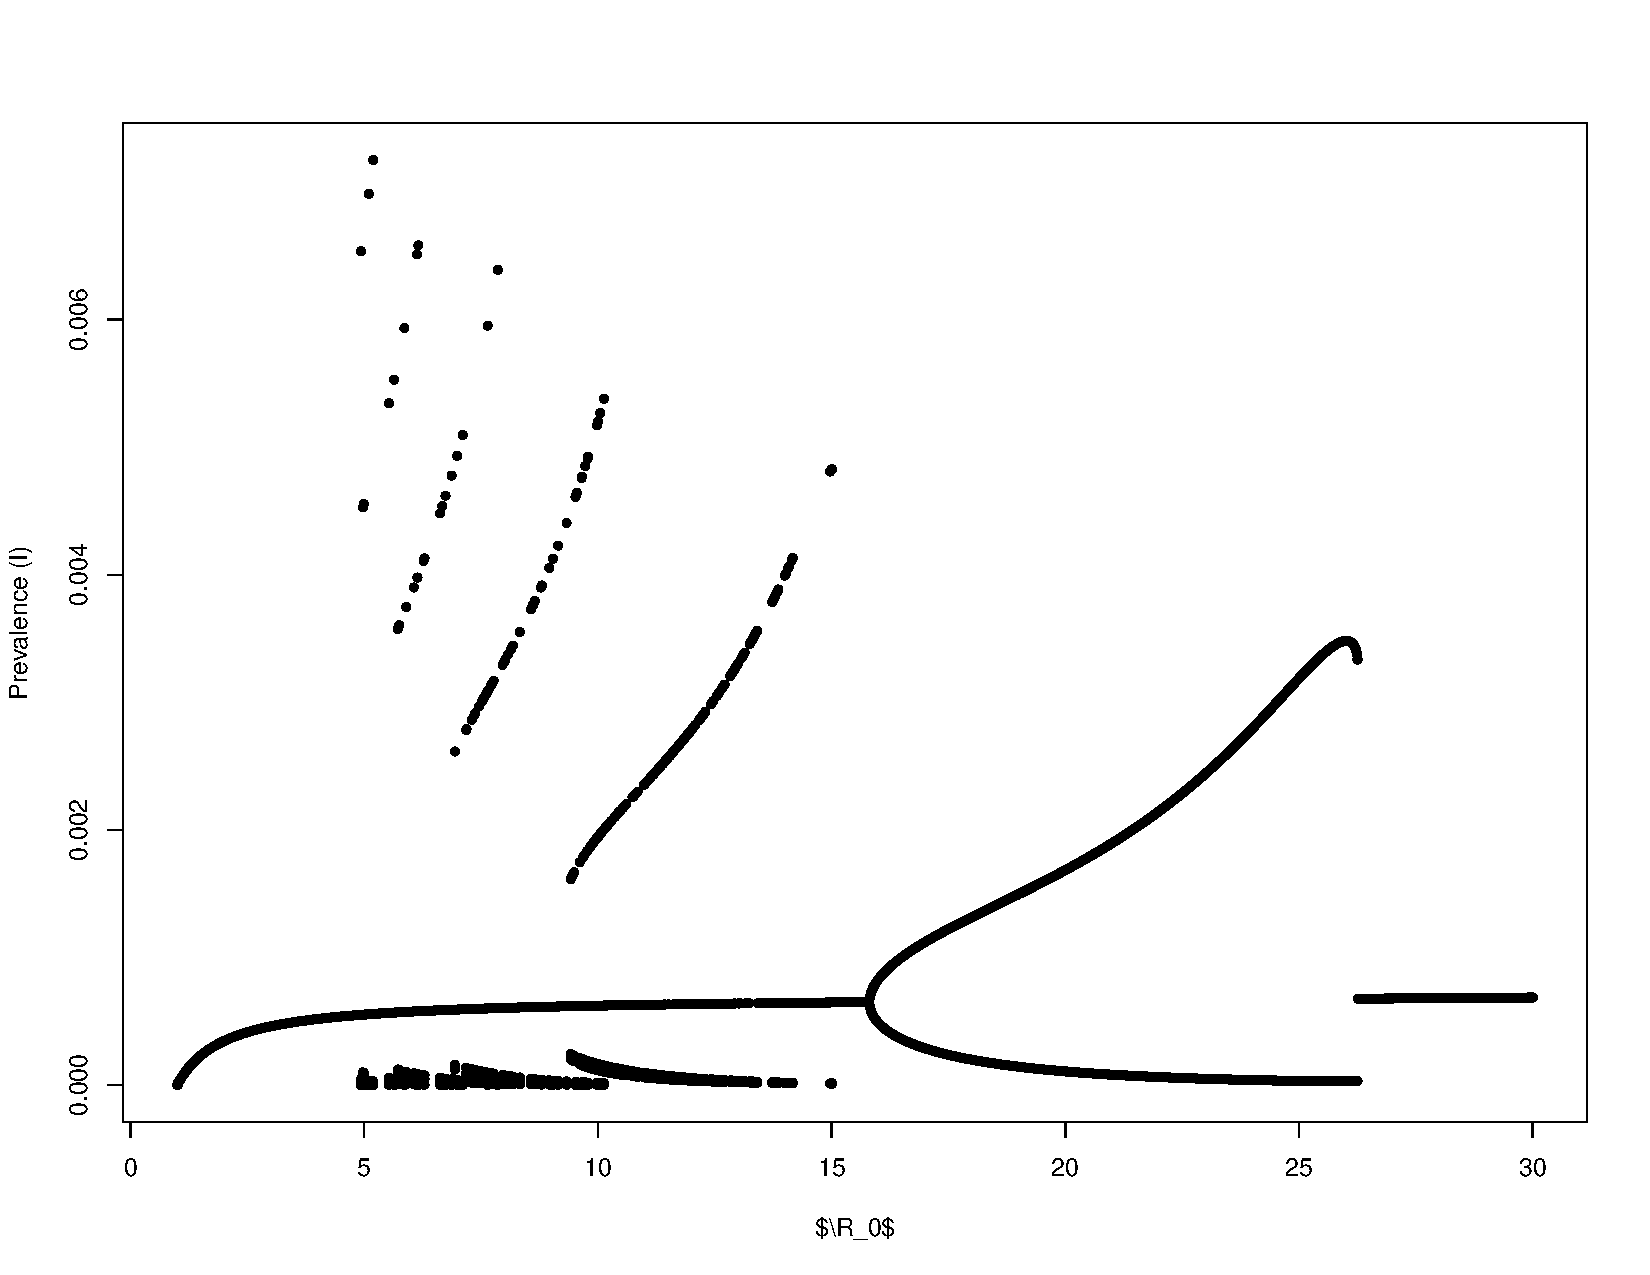
\includegraphics[width=\linewidth]{{images/bifurcation}.pdf}
\end{figure}
Further analysis of the bifurcation diagram reveal the period compositional structure. See Figure \ref{fig:period}.
\begin{figure}[H]
    \caption{The periods of the single patch sinusoidal forced SIR model vs parameter $\R_0$.}
    \label{fig:period}
    \centering
    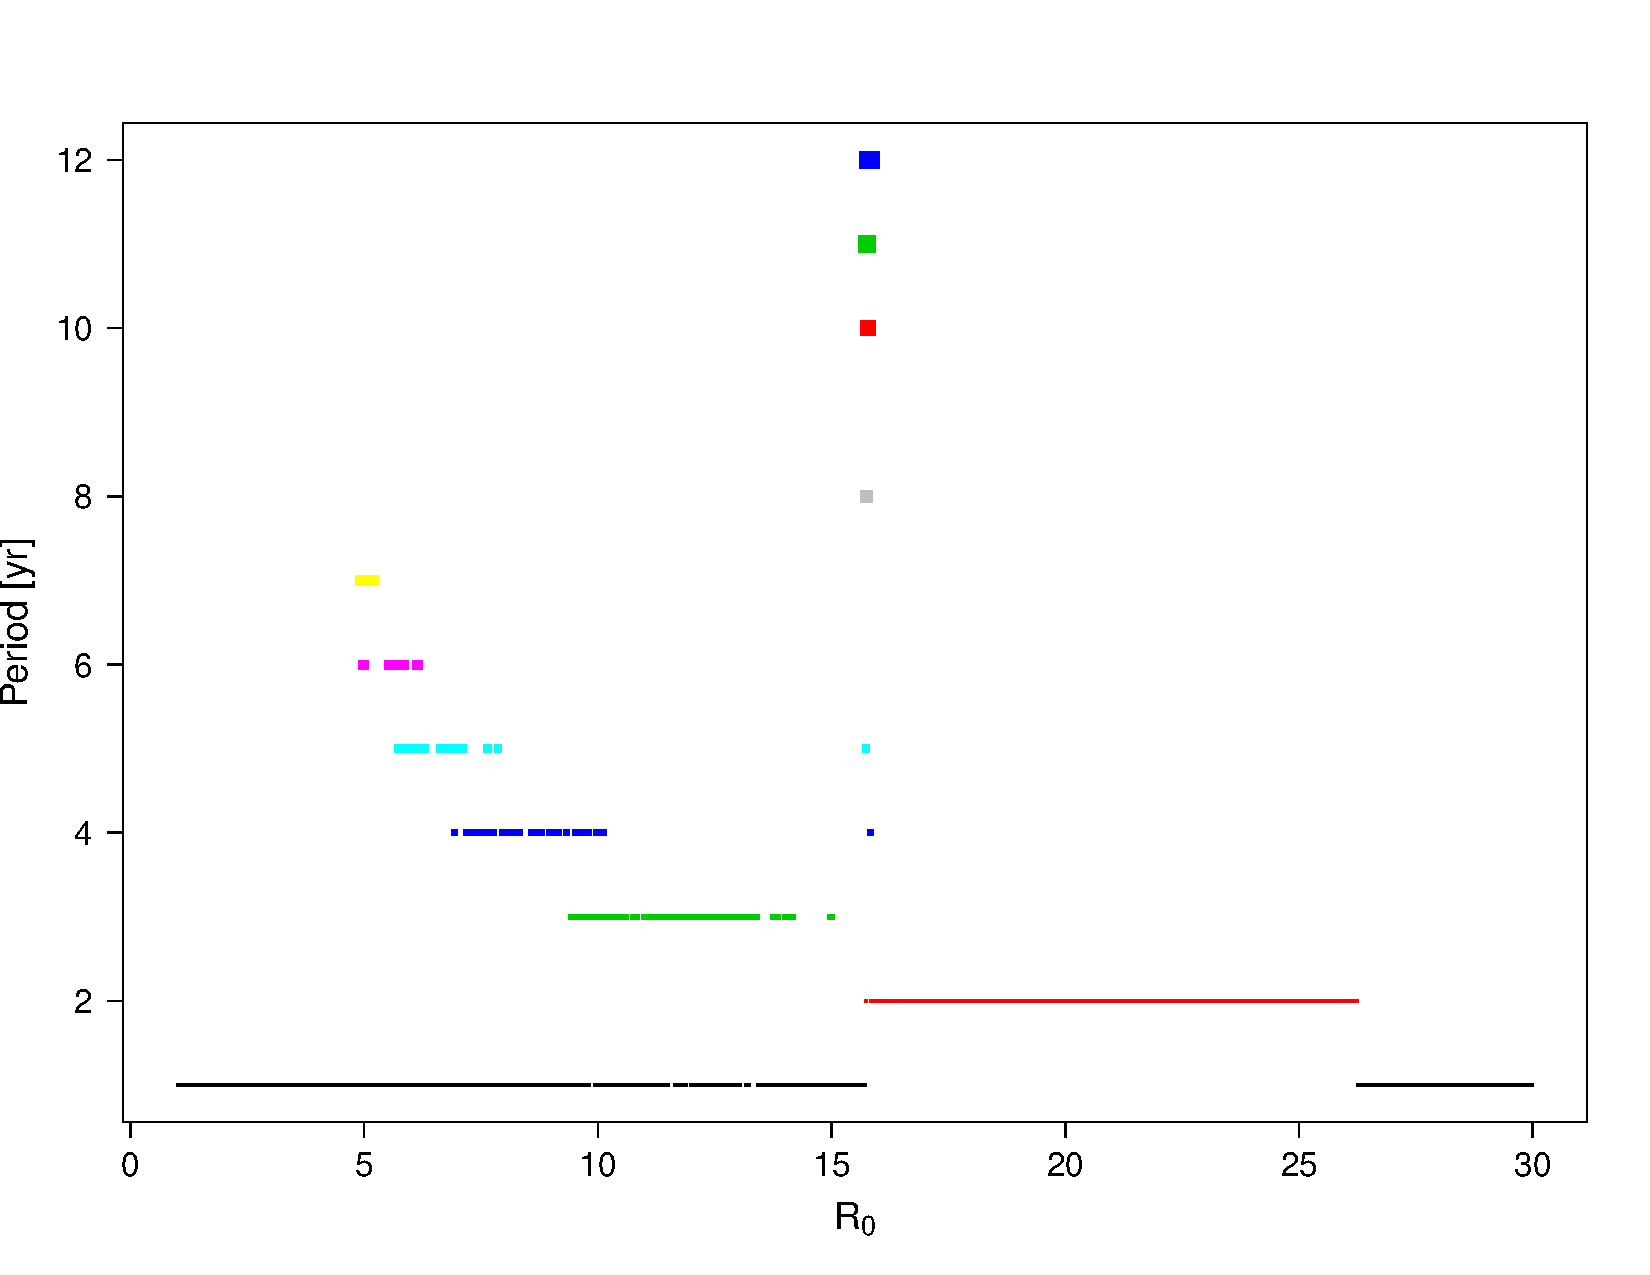
\includegraphics[width=\linewidth]{{images/period}.pdf}
\end{figure}

\begin{figure*}
    \caption{Nearest Neighbour Coupling, $\mathcal{R}_0=17$, $m=0.01$}
    \label{fig:detplotsm}
    \centering
    \subfigure[Within 30\% percent of endemic equilibrium]
    {
        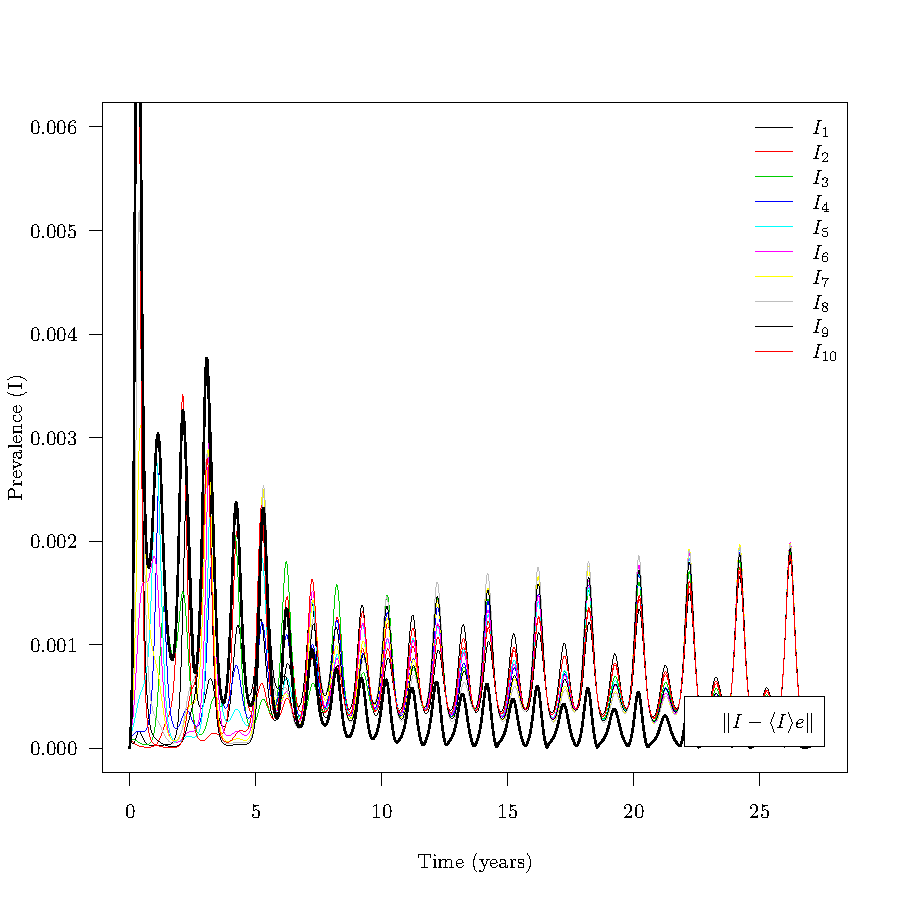
\includegraphics[width=3.0in]{{images/detNNR017m0.01}.pdf}
    }
    \subfigure[Within 40\% percent of endemic equilibrium]
    {
        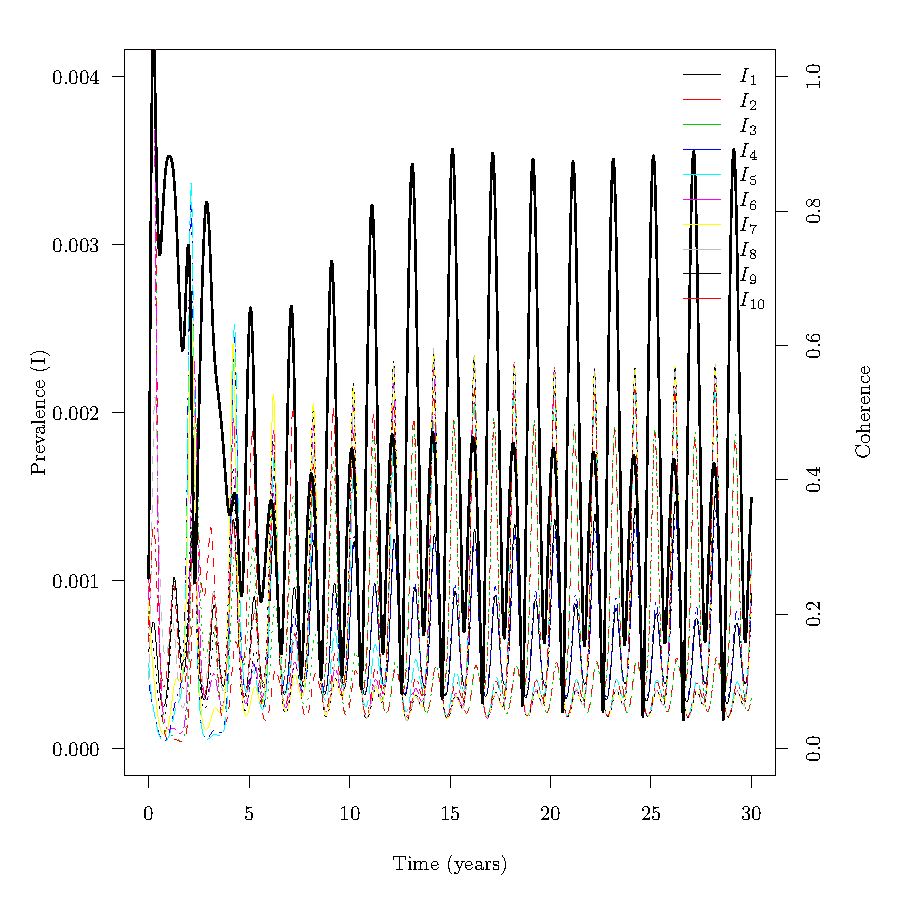
\includegraphics[width=3.0in]{{images/detNNR017m0.01wider}.pdf}
    }
    \end{figure*}

\begin{figure*}
    \caption{$\R_0=17$ and $m=0.2$}
    \label{fig:detplotsC}
    \centering
    \subfigure[Equal Coupling]
    {
        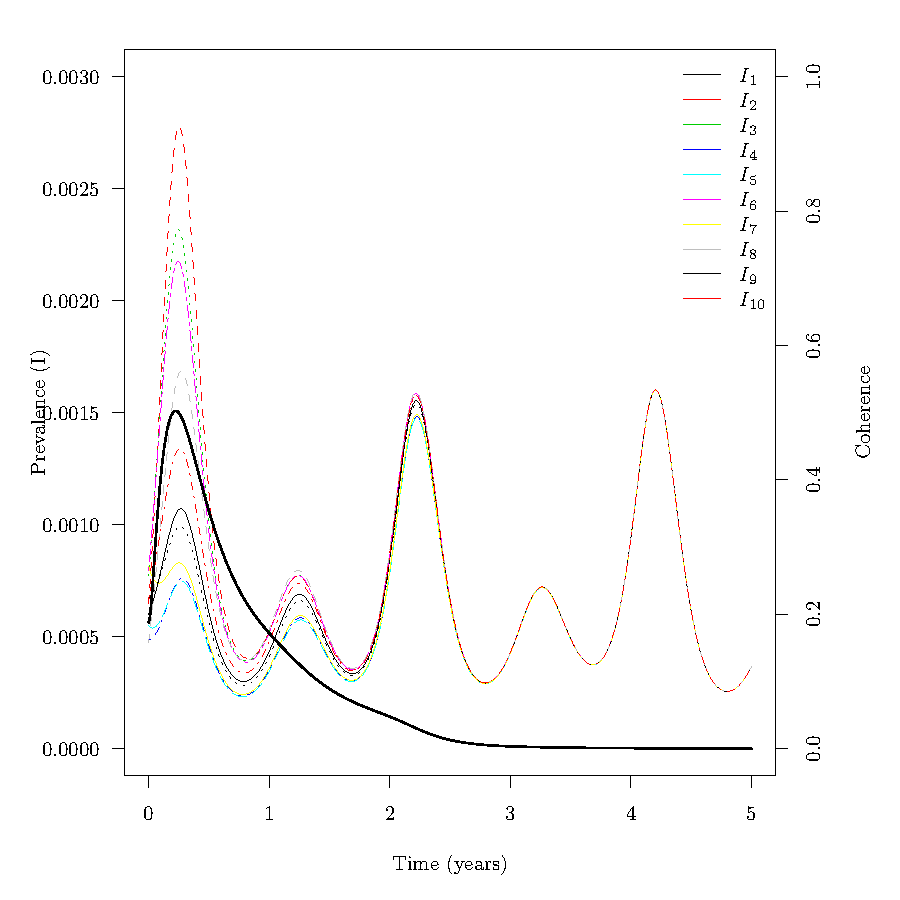
\includegraphics[width=3.0in]{{images/detECR017m0.2s}.pdf}
    }
    \subfigure[Nearest Neighbour Coupling]
    {
        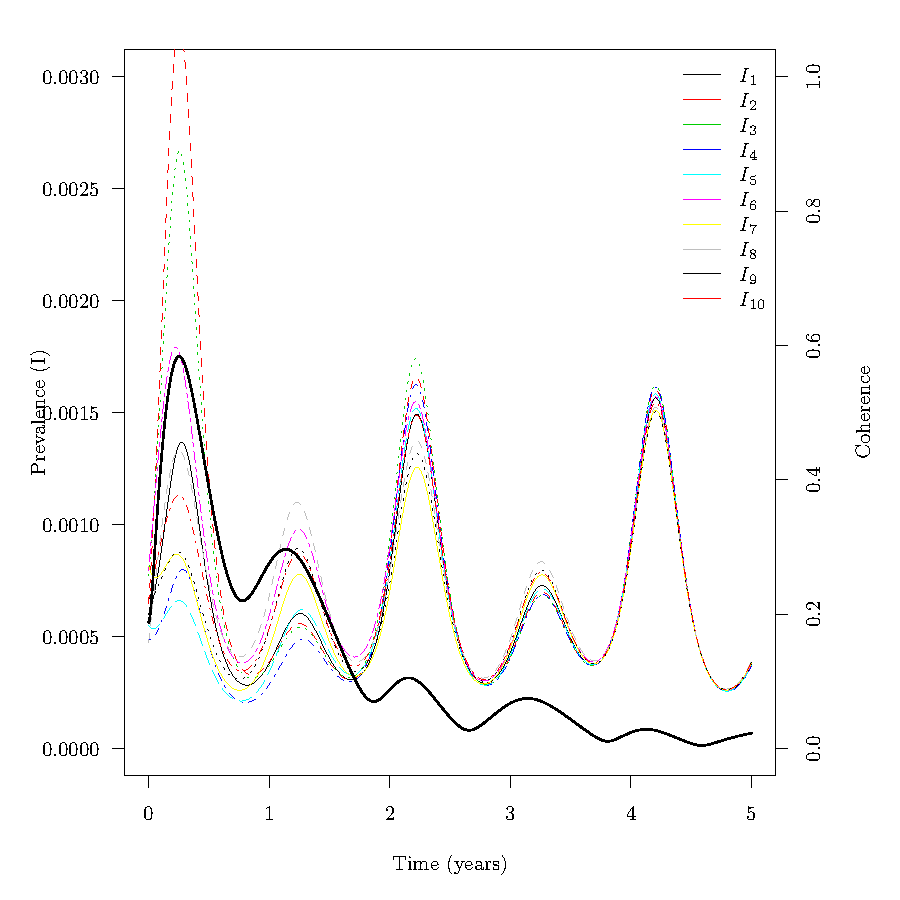
\includegraphics[width=3.0in]{{images/detNNR017m0.2s}.pdf}
    }
\end{figure*}
\begin{figure*}
    \caption{Nearest Neighbour Coupling, $m=0.2$}
    \label{fig:detplotsR0}
    \centering
    \subfigure[$\R_0=10$]
    {
        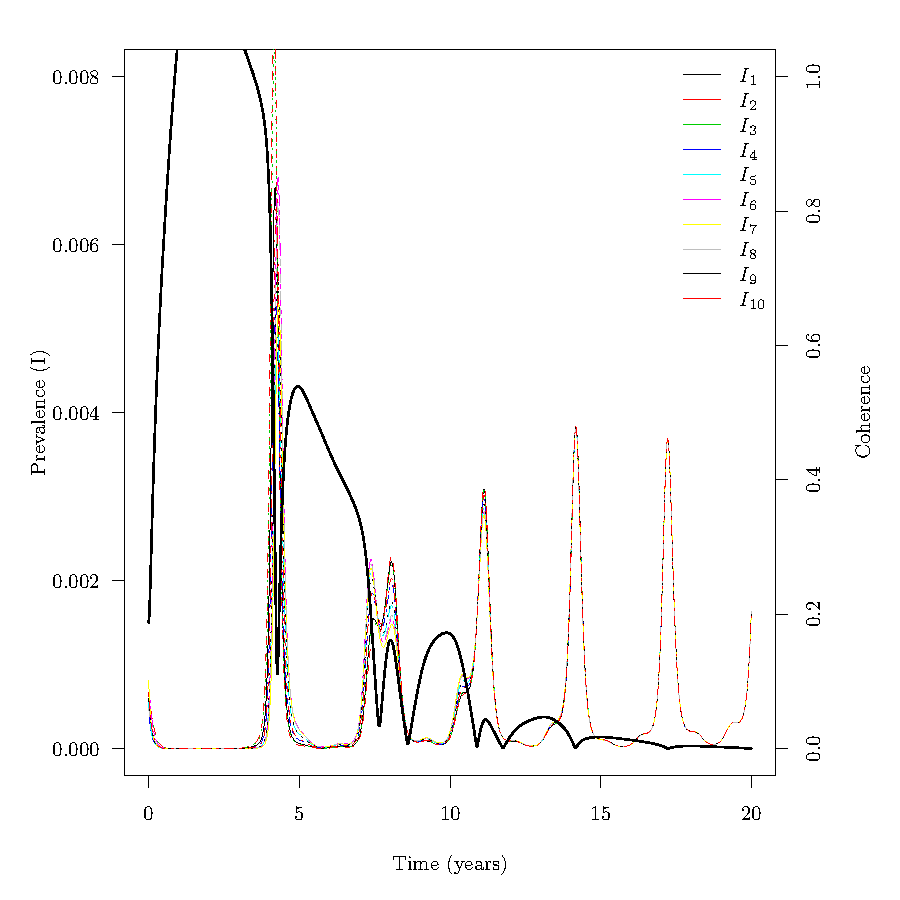
\includegraphics[width=3.0in]{{images/detNNR010m0.2}.pdf}
    }
    \subfigure[$\R_0=25$]
    {
        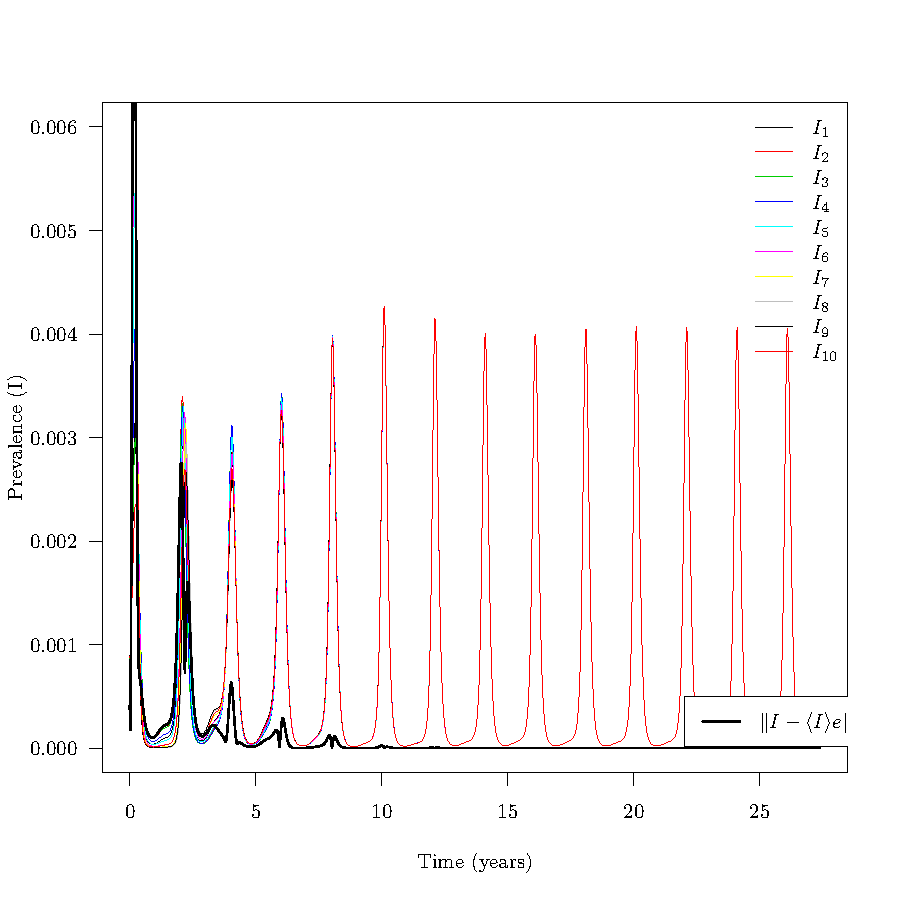
\includegraphics[width=3.0in]{{images/detNNR025m0.2}.pdf}
    }
\end{figure*}

\subsection{Deterministic Solution}
Solutions to \eqref{model} were calculated using the \Rlogo \texttt{deSolve} package. The following figures are the solutions for $n=10$, a 50 year life expectancy, a 13 day mean infectious period, nearest neighbour coupling, and seasonal forcing amplitude $\alpha = 0.1$. The initial conditions used were values within $\pm30\%$ of the $(S,I,R)$ values at the endemic equilibrium of the unforced single patch SIR model. Figure \ref{fig:detplotsm} shows the affect of the strength of connectivity, $m$***Change this. At low enough $m$ the solutions do not become coherent.

 Figure \ref{fig:detplotsR0} shows the effect $\R_0$ has on the period of oscillations and nature of the cycles.
Figure \ref{fig:detplotsC} shows the difference between equal coupling and nearest neighbour coupling. It takes longer for solutions to become coherent when using nearest neighbour coupling.


\begin{figure*}
    \caption{An exact stochastic simulation using the Gillespie algorithm.}
    \label{fig:Gillplot}
    \centering
    \subfigure[Population of 3,000 per patch]
    {
        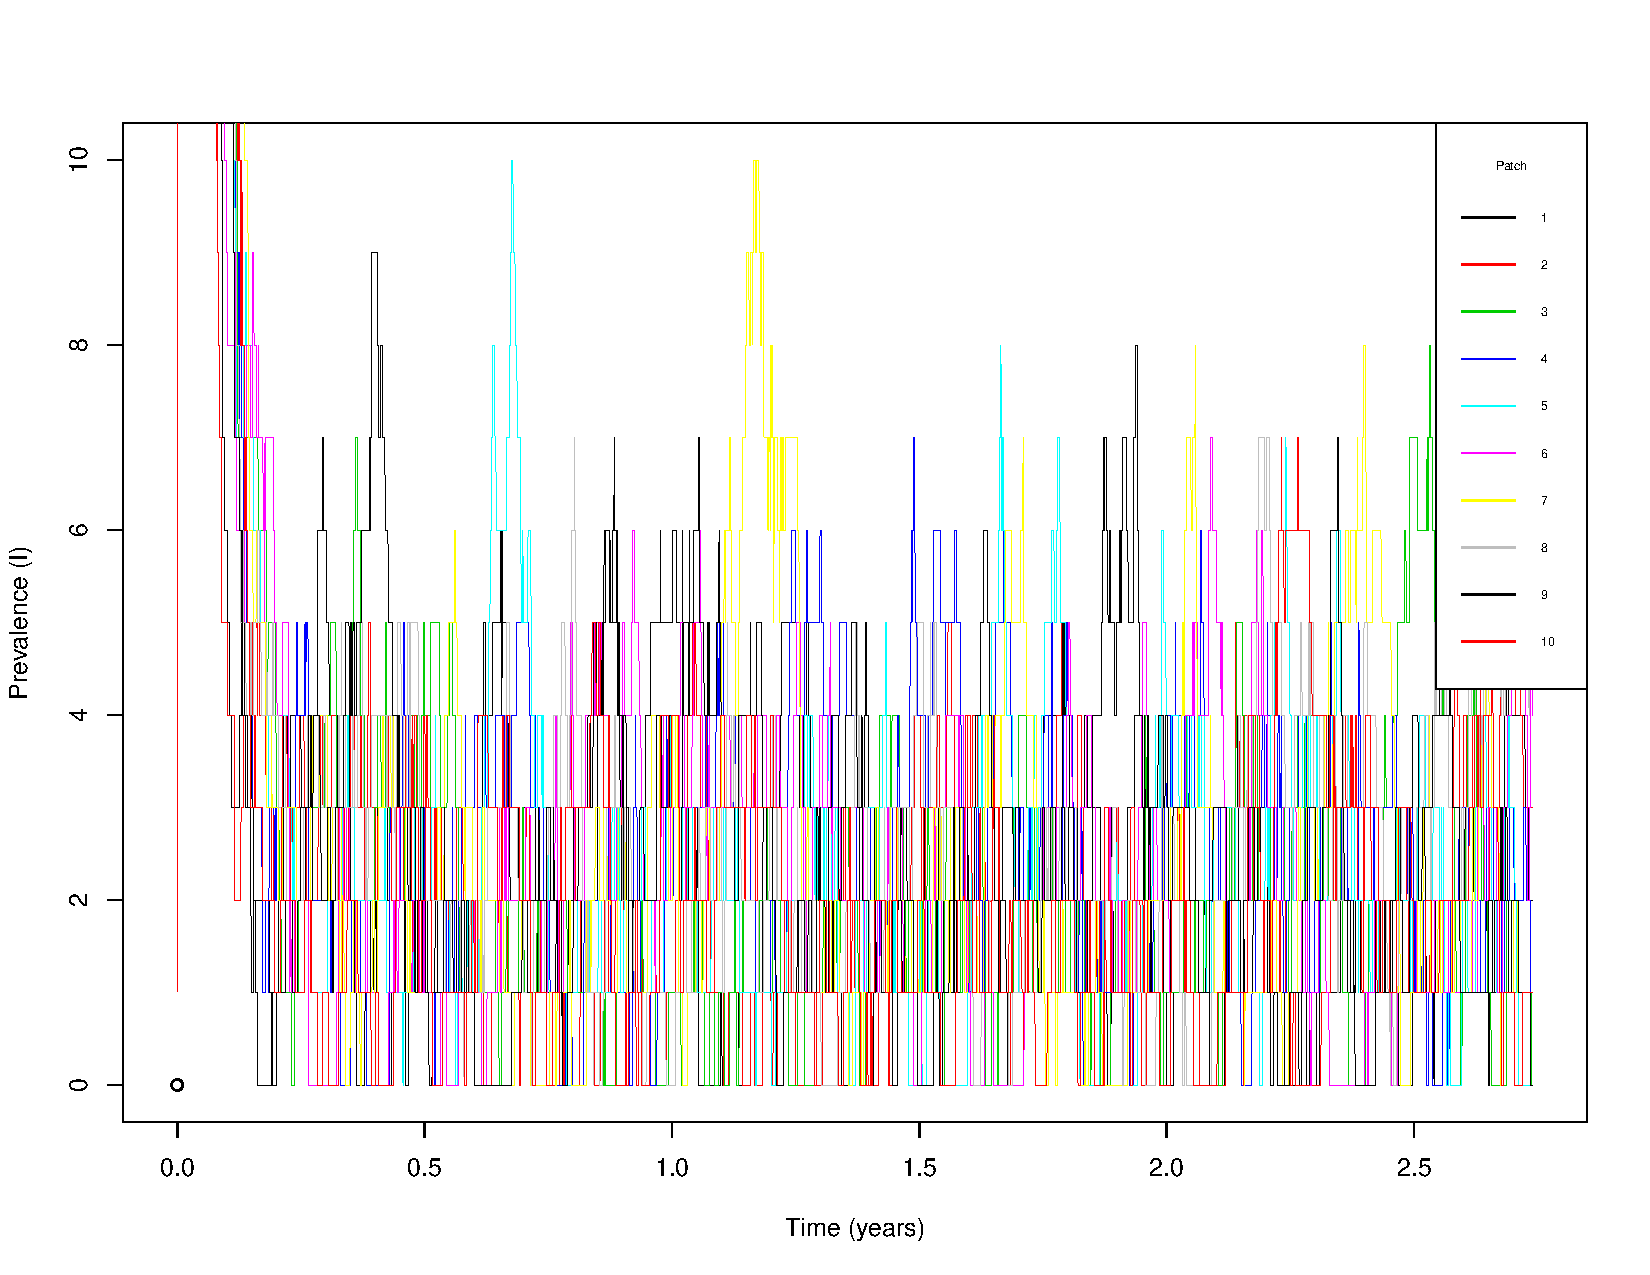
\includegraphics[width=3.0in]{{images/GillECR017m0.2small}.pdf}
    }
    \subfigure[Population of 250,000 per patch]
    {
        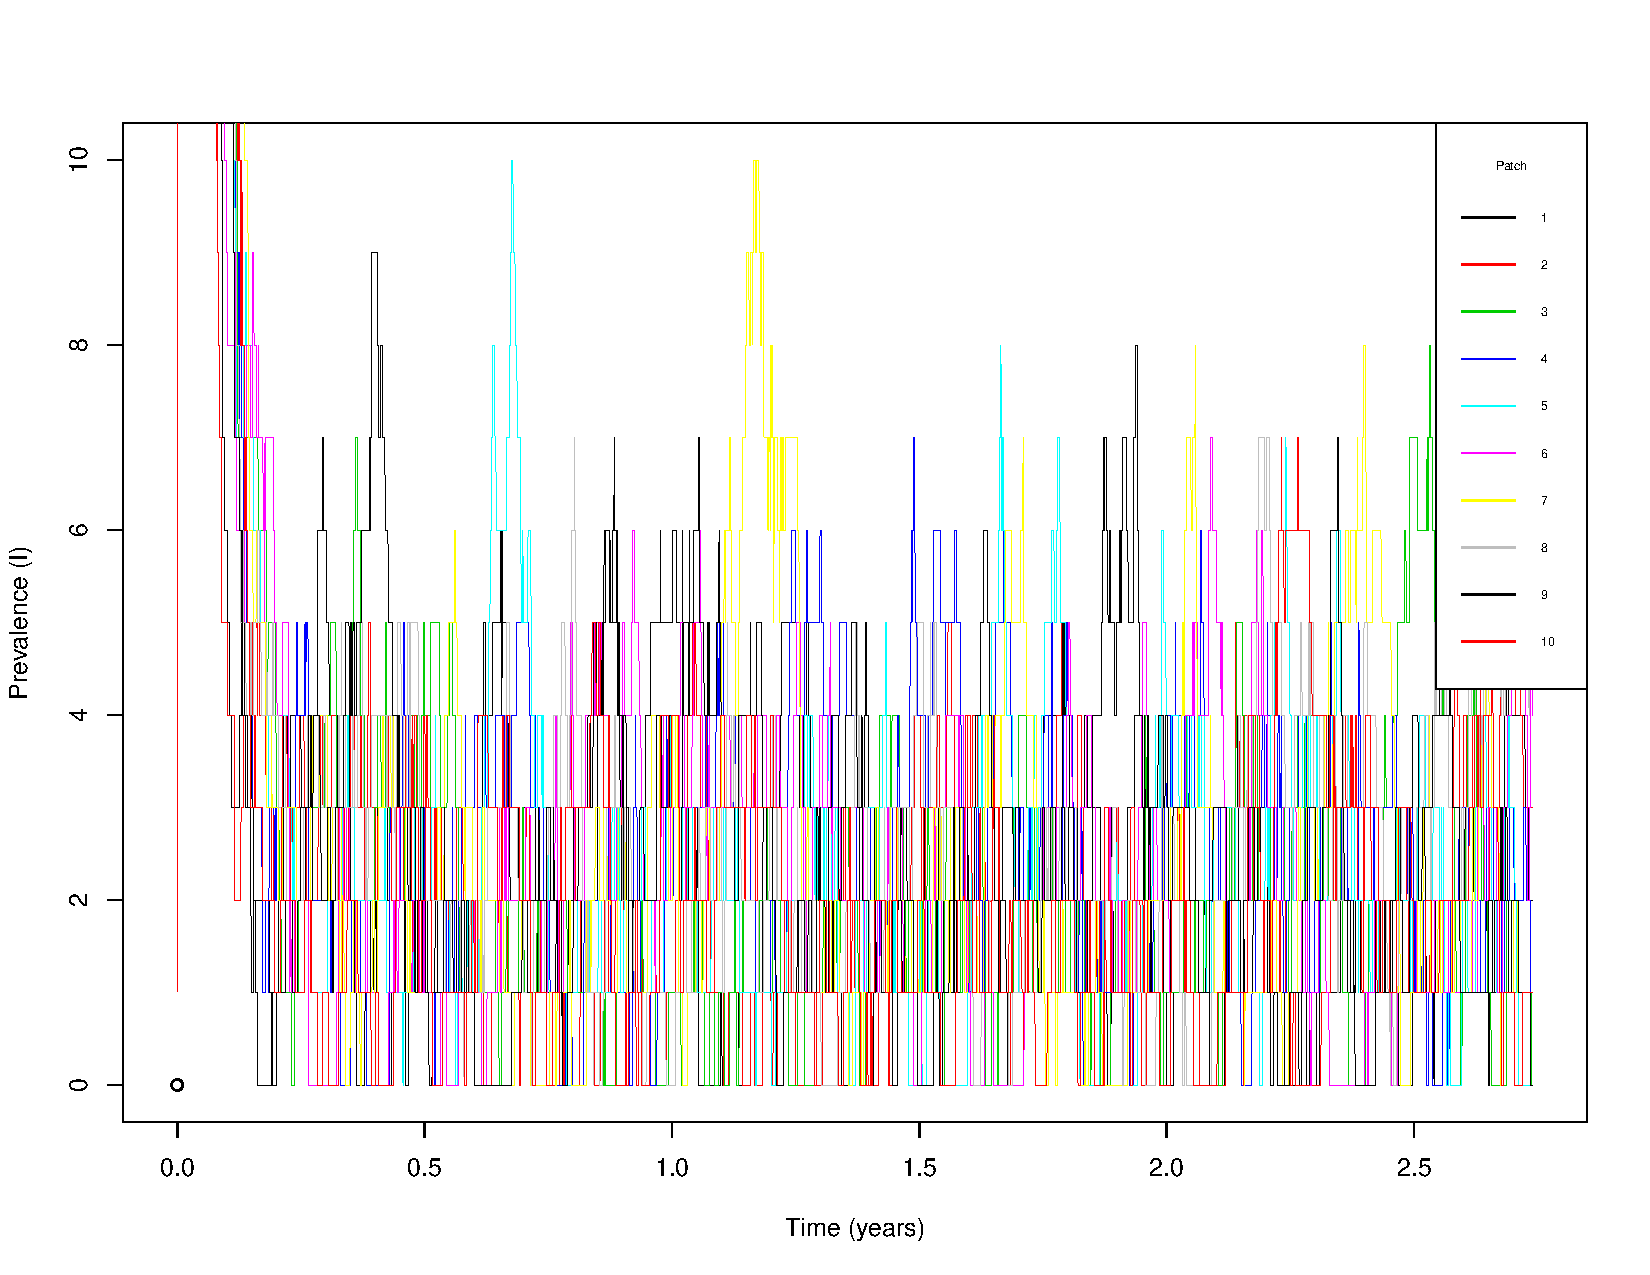
\includegraphics[width=3.0in]{{images/GillECR017m0.2}.pdf}
    }
\end{figure*}


\subsection{Stochastic Simulations} 
A stochastic version of this model was simulated exactly using the Gillespie algorithm with the same parameters and similar initial conditions used for the deterministic solution. Equal coupling and $R_0=17$ and $m=0.5$ were used. See Figure \ref{fig:Gillplot}. \par
For larger population sizes, approximate stochastic simulations (using the \Rlogo \verb|adaptivetau| package) were used. See Figure \ref{fig:adapplot} for a simulation with population of 500,000.

\begin{figure}[h]
    \caption{An approximate stochastic simulation using the adaptive tau-leaping method}
    \label{fig:adapplot}
    \centering
    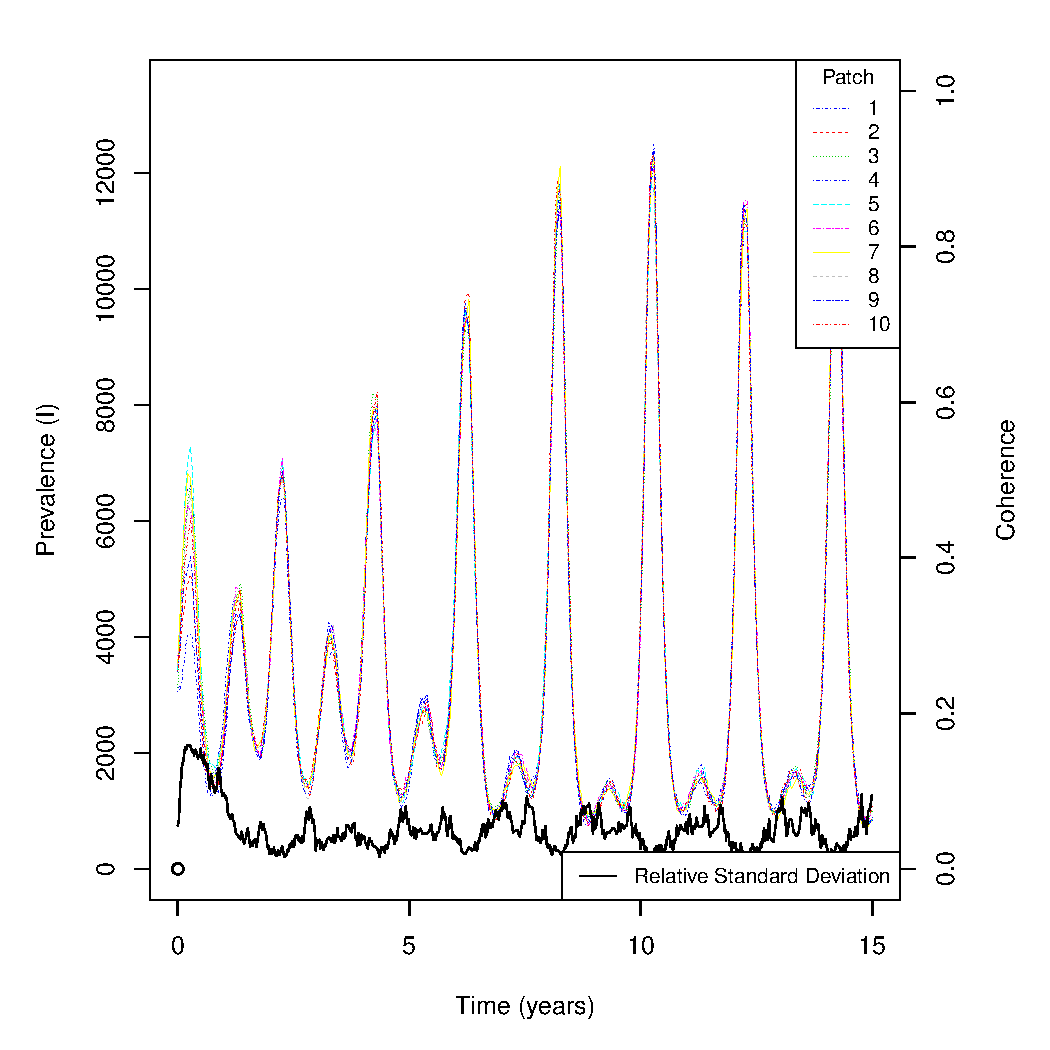
\includegraphics[width=\linewidth]{{images/adaptauECR017m0.2}.pdf}
\end{figure}

\subsection{Coherence Dependence Parameters} 

\section{Discussion} 
\section{Conclusion } 

\onecolumn
\addcontentsline{toc}{section}{\protect\numberline{}Bibilography}%
\bibliographystyle{unsrt}
\bibliography{ModelStudents} 
\end{document}